\documentclass[12pt,letterpaper]{article}
\usepackage{graphicx,textcomp}
\usepackage{natbib}
\usepackage{setspace}
\usepackage{fullpage}
\usepackage{color}
\usepackage[reqno]{amsmath}
\usepackage{amsthm}
\usepackage{fancyvrb}
\usepackage{amssymb,enumerate}
\usepackage[all]{xy}
\usepackage{endnotes}
\usepackage{lscape}
\newtheorem{com}{Comment}
\usepackage{float}
\usepackage{hyperref}
\newtheorem{lem} {Lemma}
\newtheorem{prop}{Proposition}
\newtheorem{thm}{Theorem}
\newtheorem{defn}{Definition}
\newtheorem{cor}{Corollary}
\newtheorem{obs}{Observation}
\usepackage[compact]{titlesec}
\usepackage{dcolumn}
\usepackage{tikz}
\usetikzlibrary{arrows}
\usepackage{multirow}
\usepackage{xcolor}
\newcolumntype{.}{D{.}{.}{-1}}
\newcolumntype{d}[1]{D{.}{.}{#1}}
\definecolor{light-gray}{gray}{0.65}
\usepackage{url}
\usepackage{listings}
\usepackage{color}

\definecolor{codegreen}{rgb}{0,0.6,0}
\definecolor{codegray}{rgb}{0.5,0.5,0.5}
\definecolor{codepurple}{rgb}{0.58,0,0.82}
\definecolor{backcolour}{rgb}{0.95,0.95,0.92}

\lstdefinestyle{mystyle}{
	backgroundcolor=\color{backcolour},   
	commentstyle=\color{codegreen},
	keywordstyle=\color{magenta},
	numberstyle=\tiny\color{codegray},
	stringstyle=\color{codepurple},
	basicstyle=\footnotesize,
	breakatwhitespace=false,         
	breaklines=true,                 
	captionpos=b,                    
	keepspaces=true,                 
	numbers=left,                    
	numbersep=5pt,                  
	showspaces=false,                
	showstringspaces=false,
	showtabs=false,                  
	tabsize=2
}
\lstset{style=mystyle}
\newcommand{\Sref}[1]{Section~\ref{#1}}
\newtheorem{hyp}{Hypothesis}

\title{Applied Stats - Problem Set 1}
\author{Yana Konshyna}


\begin{document}
	\maketitle
	
	\section*{Instructions}
	\begin{itemize}
	\item Please show your work! You may lose points by simply writing in the answer. If the problem requires you to execute commands in \texttt{R}, please include the code you used to get your answers. Please also include the \texttt{.R} file that contains your code. If you are not sure if work needs to be shown for a particular problem, please ask.
\item Your homework should be submitted electronically on GitHub.
\item This problem set is due before 23:59 on Sunday October 1, 2023. No late assignments will be accepted.
\item Total available points for this homework is 80.
	\end{itemize}
	
	\vspace{1cm}
	\section*{Question 1 (40 points): Education}

A school counselor was curious about the average of IQ of the students in her school and took a random sample of 25 students' IQ scores. The following is the data set:\\


\lstinputlisting[language=R, firstline=36, lastline=36]{PS01_answers_YK_23359606.R}  

\vspace{1cm}

\begin{enumerate}
	\item Find a 90\% confidence interval for the average student IQ in the school.\\
	
	\item Next, the school counselor was curious  whether  the average student IQ in her school is higher than the average IQ score (100) among all the schools in the country.\\ 
	
	\noindent Using the same sample, conduct the appropriate hypothesis test with $\alpha=0.05$.
\end{enumerate}

\newpage
\section*{Answers to Question 1: Education}

\noindent 1. \textbf{Code in R:}
\lstinputlisting[language=R, firstline=39, lastline=56]{PS01_answers_YK_23359606.R}  
\vspace{.25cm}

\noindent \textbf{Output: }
\begin{verbatim}
> length(y)
[1] 25
> mean(y)
[1] 98.44
> sd(y)/sqrt(length(y)) 
[1] 2.618575
> # Finding confidence interval using t distribution, because n<30
> # critical value
> t_score <- qt(0.95, df=length(y)-1) 
> #margin of error
> me<-(t_score)*(sd(y)/sqrt(length(y)))
> # Lower bound, 90 confidence level
> lower_90_t <- mean(y)-me
> # Upper bound, 90 confidence level
> upper_90_t <- mean(y)+me
> #Print result
> conf_int90 <- c(lower_90_t, upper_90_t)
> conf_int90
[1]  93.95993 102.92007
\end{verbatim}
\vspace{.25cm}

\noindent \textbf{Conclusion:} For finding a 90\% confidence interval for the average student IQ in the school I used the t distribution, because n less than 30. As result, 90\% confidence interval is [93.95993, 102.92007].


\newpage
\noindent 2. I set null hypothesis H0: the average student IQ in school is equal to the average IQ score (100) among all the schools in the country. Alternative hypothesis Ha: the average student IQ in school is greater than 100.


\lstinputlisting[language=R, firstline=58, lastline=59]{PS01_answers_YK_23359606.R}  

\noindent \textbf{Output:} 
\begin{verbatim}
One Sample t-test

data:  y
t = -0.59574, df = 24, p-value = 0.7215
alternative hypothesis: true mean is greater than 100
95 percent confidence interval:
93.95993      Inf
sample estimates:
mean of x 
98.44  
\end{verbatim}


\noindent Conclusion: P-value = 0.7215. It is greater than $\alpha=0.05$, so I cannot reject null hypothesis. I don't have a significant evidence that the average student IQ in school is higher than the average IQ score (100) among all the schools in the country.
\newpage

	\section*{Question 2 (40 points): Political Economy}

\noindent Researchers are curious about what affects the amount of money communities spend on addressing homelessness. The following variables constitute our data set about social welfare expenditures in the USA. \\
\vspace{.5cm}


\begin{tabular}{r|l}
	\texttt{State} &\emph{50 states in US} \\
	\texttt{Y} & \emph{per capita expenditure on shelters/housing assistance in state}\\
	\texttt{X1} &\emph{per capita personal income in state} \\
	\texttt{X2} &  \emph{Number of residents per 100,000 that are "financially insecure" in state}\\
	\texttt{X3} &  \emph{Number of people per thousand residing in urban areas in state} \\
	\texttt{Region} &  \emph{1=Northeast, 2= North Central, 3= South, 4=West} \\
\end{tabular}

\vspace{.5cm}
\noindent Explore the \texttt{expenditure} data set and import data into \texttt{R}.
\vspace{.5cm}
\lstinputlisting[language=R, firstline=65, lastline=65]{PS01_answers_YK_23359606.R}  
\vspace{.5cm}
\begin{itemize}

\item
Please plot the relationships among \emph{Y}, \emph{X1}, \emph{X2}, and \emph{X3}? What are the correlations among them (you just need to describe the graph and the relationships among them)?
\vspace{.5cm}
\item
Please plot the relationship between \emph{Y} and \emph{Region}? On average, which region has the highest per capita expenditure on housing assistance?
\vspace{.5cm}
\item
Please plot the relationship between \emph{Y} and \emph{X1}? Describe this graph and the relationship. Reproduce the above graph including one more variable \emph{Region} and display different regions with different types of symbols and colors.
\end{itemize}

\newpage
\section*{Answers to Question 2: Political Economy}

\noindent 1.1. The relationships between \emph{Y} and \emph{X1}:
\lstinputlisting[language=R, firstline=71, lastline=77]{PS01_answers_YK_23359606.R}  

\noindent Scatterplot 1.

\begin{figure}[h!]\centering
	\caption{\footnotesize }
	\label{fig:plot_1}
	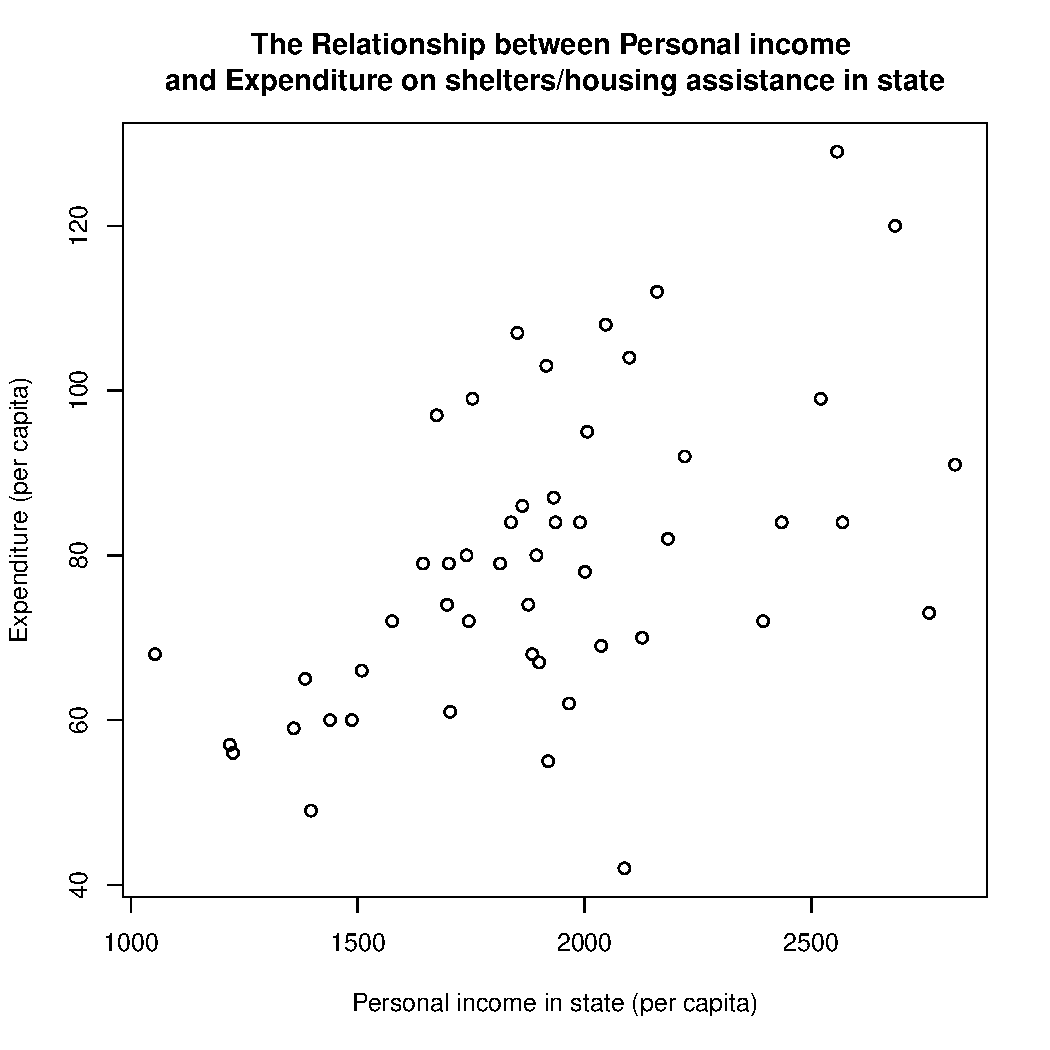
\includegraphics[width=.75\textwidth]{plot1_1.pdf}
\end{figure}

\noindent \textbf{Conclusion:} The scatterplot has a positive linear correlation. It shows a tendency for state with higher personal income to have higher levels of expenditure on shelters/housing assistance (per capita). 
\vspace{.5cm}

\newpage
\noindent 1.2. The relationships between \emph{Y} and \emph{X2}:
\lstinputlisting[language=R, firstline=80, lastline=87]{PS01_answers_YK_23359606.R}  

\noindent Scatterplot 2.
\begin{figure}[h!]\centering
	\caption{\footnotesize }
	\label{fig:plot_1}
	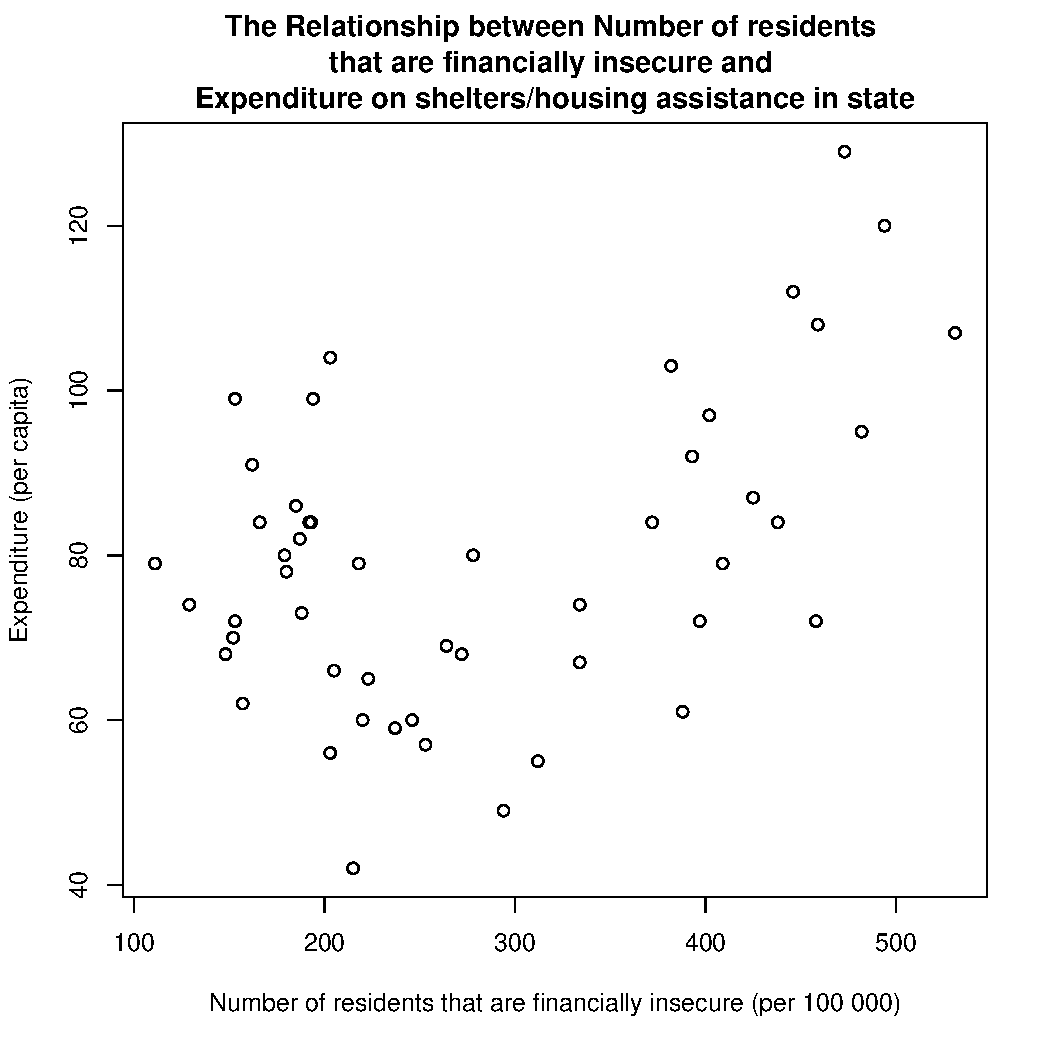
\includegraphics[width=.75\textwidth]{plot1_2.pdf}
\end{figure}

\noindent \textbf{Conclusion:} The scatterplot has a positive linear correlation. It shows a tendency for state with higher number of residents that are "financially insecure" to have the higher levels of expenditure on shelters/housing assistance (per capita).
\vspace{.5cm}

\newpage
\noindent 1.3. The relationships between \emph{Y} and \emph{X3}:
\lstinputlisting[language=R, firstline=90, lastline=96]{PS01_answers_YK_23359606.R}  

\noindent Scatterplot 3. 
\begin{figure}[h!]\centering
	\caption{\footnotesize }
	\label{fig:plot_1}
	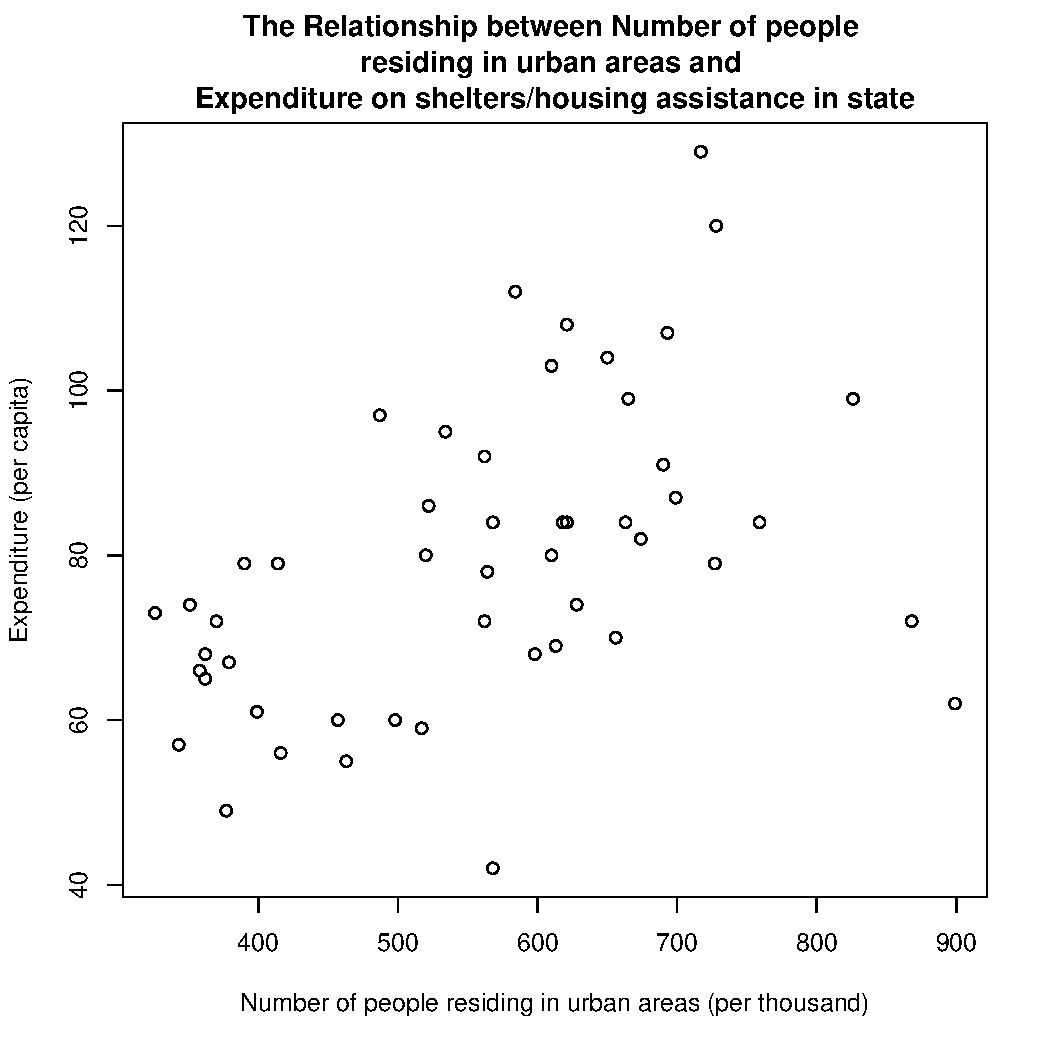
\includegraphics[width=.75\textwidth]{plot1_3.pdf}
\end{figure}

\noindent \textbf{Conclusion: } The scatterplot has a positive linear correlation. It shows a tendency for state with higher number of people residing in urban areas to have higher levels of expenditure on shelters/housing assistance (per capita).
\vspace{.5cm}

\newpage
\noindent 1.4. The relationships between \emph{X1} and \emph{X2}:
\lstinputlisting[language=R, firstline=99, lastline=105]{PS01_answers_YK_23359606.R} 
 
\noindent Scatterplot 4. 
\begin{figure}[h!]\centering
	\caption{\footnotesize }
	\label{fig:plot_1}
	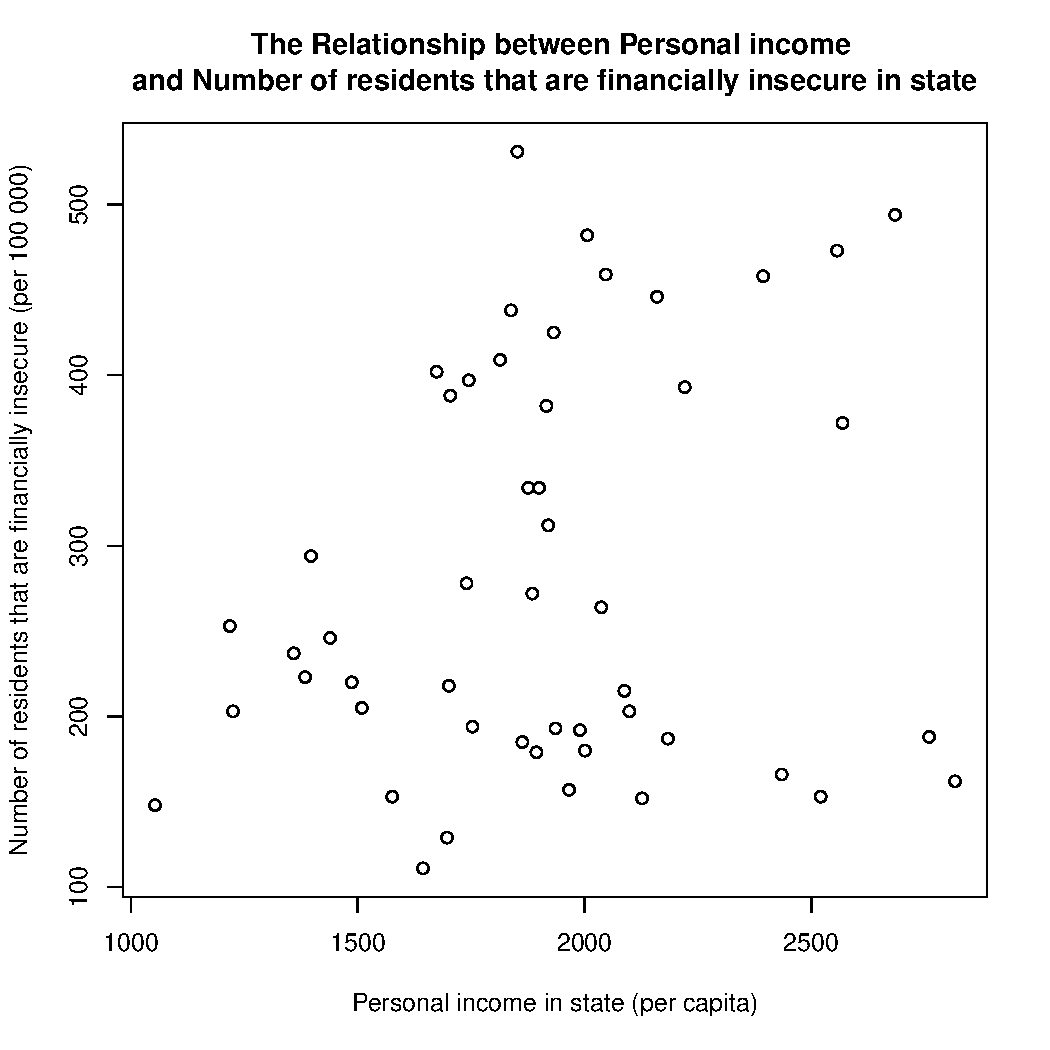
\includegraphics[width=.75\textwidth]{plot1_4.pdf}
\end{figure}

\noindent \textbf{Conclusion:} The scatterplot shows that a tendency for state with  number of people who have middle and higher personal income to have higher levels of number of residents that are "financially insecure".
\vspace{.5cm}

\newpage
\noindent 1.5. The relationships between \emph{X1} and \emph{X3}:
\lstinputlisting[language=R, firstline=108, lastline=114]{PS01_answers_YK_23359606.R} 
 
\noindent Scatterplot 5. 
\begin{figure}[h!]\centering
	\caption{\footnotesize }
	\label{fig:plot_1}
	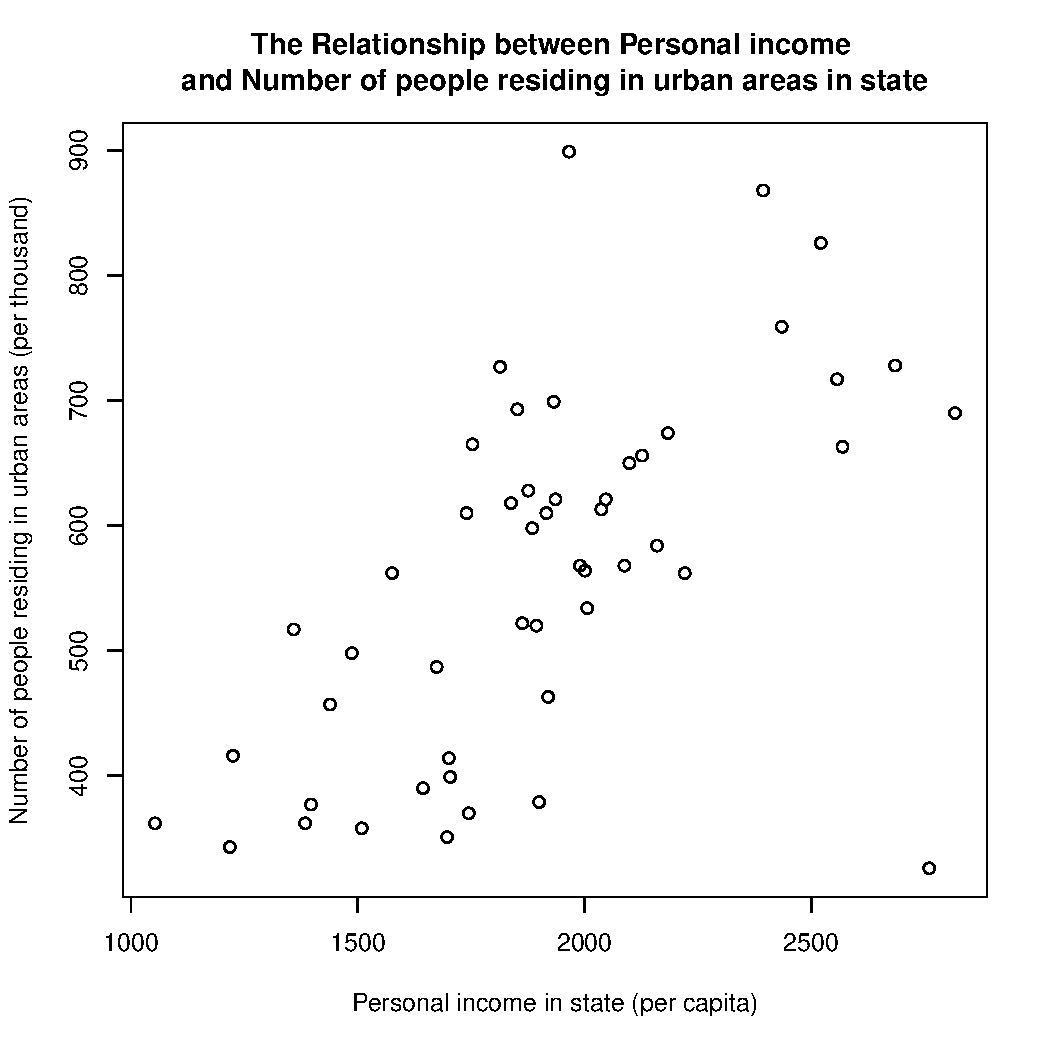
\includegraphics[width=.75\textwidth]{plot1_5.pdf}
\end{figure}

\noindent \textbf{Conclusion:} The scatterplot has a positive linear correlation. It shows a tendency for state with higher personal income to have higher number of people residing in urban areas. 
\vspace{.5cm}

\newpage
\noindent 1.6. The relationships between \emph{X2} and \emph{X3}:
\lstinputlisting[language=R, firstline=117, lastline=123]{PS01_answers_YK_23359606.R}  

\noindent Scatterplot 6. 
\vspace{.5cm}

\begin{figure}[h!]\centering
	\caption{\footnotesize }
	\label{fig:plot_1}
	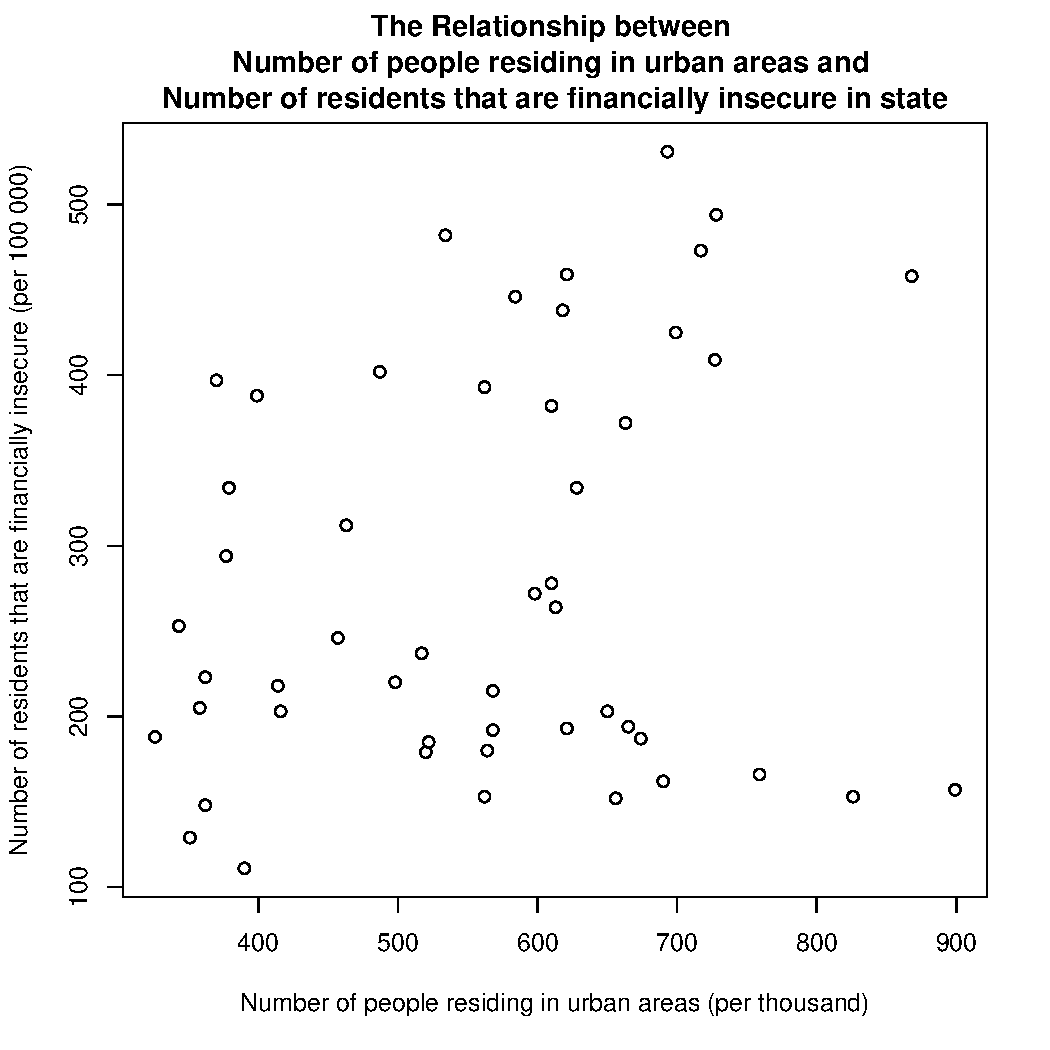
\includegraphics[width=.75\textwidth]{plot1_6.pdf}
\end{figure}

\noindent \textbf{Conclusion:} The scatterplot shows a tendency for state with low and middle number of people residing in urban area to have higher number of of residents that are "financially insecure".
\vspace{.5cm}

\newpage
\noindent 2. The relationship between \emph{Y} and \emph{Region}:
\lstinputlisting[language=R, firstline=126, lastline=132]{PS01_answers_YK_23359606.R}  

\noindent Scatterplot 7.
\vspace{.5cm} 

\begin{figure}[h!]\centering
	\caption{\footnotesize }
	\label{fig:plot_1}
	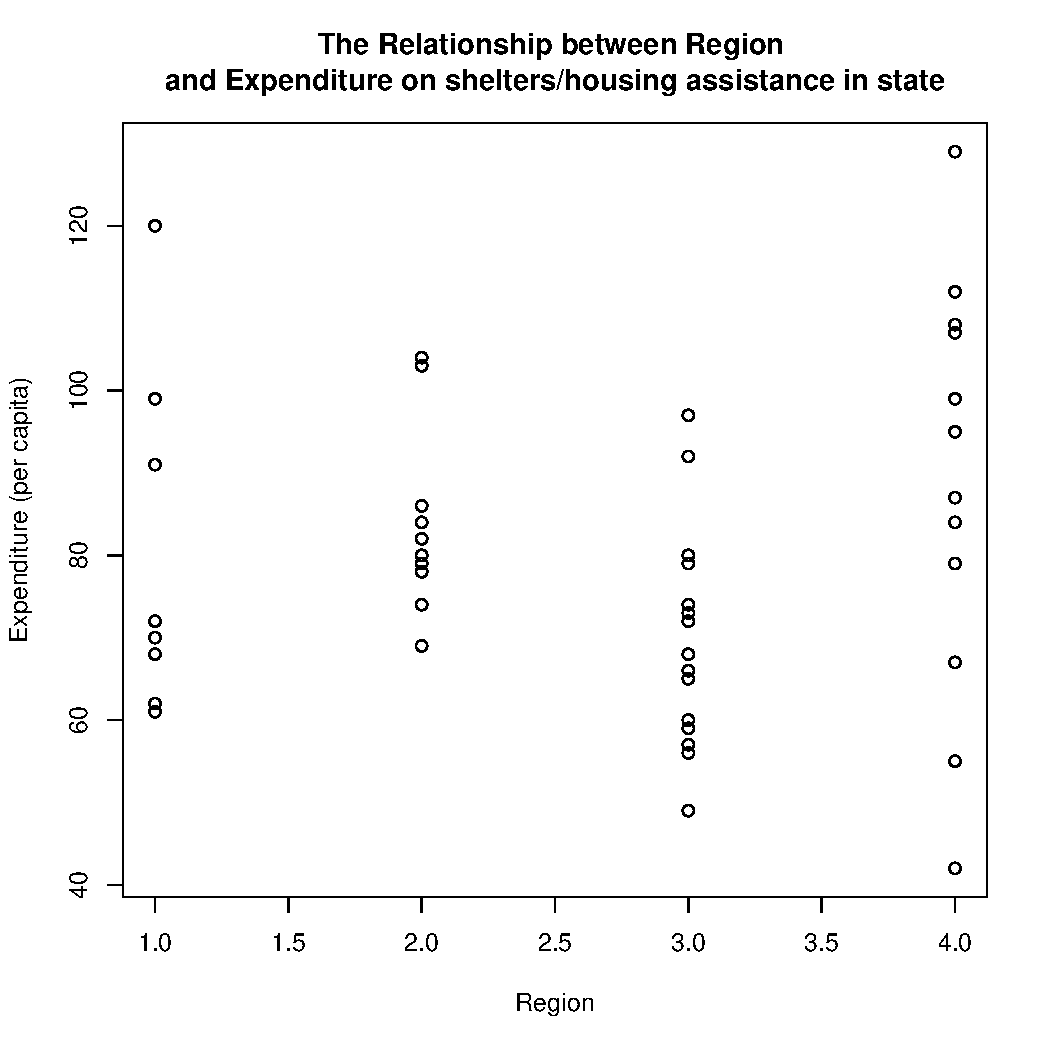
\includegraphics[width=.75\textwidth]{plot2_1.pdf}
\end{figure}

\noindent \textbf{Conclusion:} The scatterplot shows that on average regions 1 and 4 have the highest expenditure on shelters/housing assistance in state (per capita). Rigion 3 has the lowest expenditure on shelters/housing assistance in state (per capita)

\newpage
\noindent 3. The relationship between \emph{Y} and \emph{X1} including one more variable \emph{Region}:
\lstinputlisting[language=R, firstline=134, lastline=145]{PS01_answers_YK_23359606.R}  

\noindent Scatterplot 8. 

\begin{figure}[h!]\centering
	\caption{\footnotesize }
	\label{fig:plot_1}
	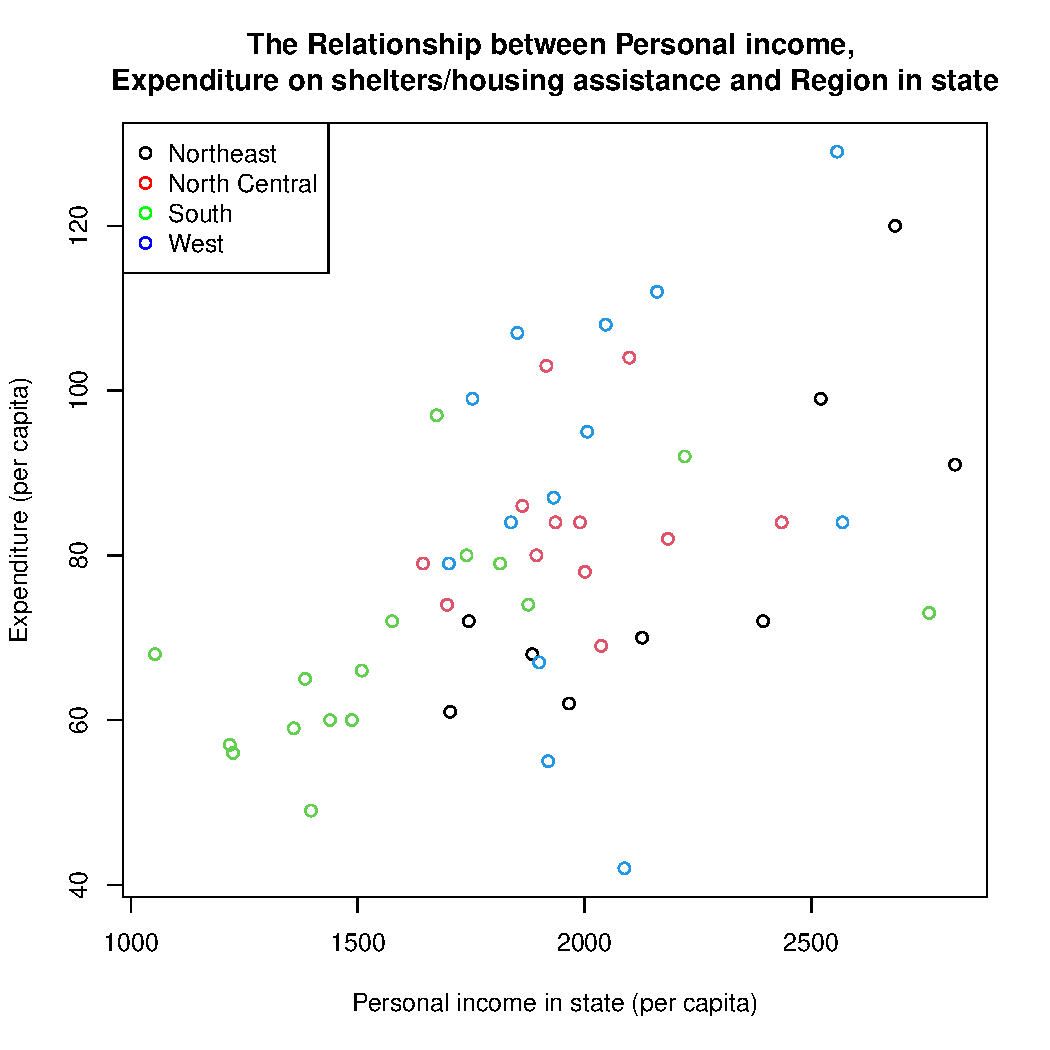
\includegraphics[width=.75\textwidth]{plot3_1.pdf}
\end{figure}

\noindent \textbf{Conclusion:} The scatterplot has a positive linear correlation. It shows a tendency for state with higher personal income to have higher levels of expenditure on shelters/housing assistance (per capita). Especially in the two region: West and Northeast. South region has lowest level of expenditure on shelters/housing assistance (per capita).
\vspace{.5cm} 

\end{document}
